\documentclass{article}
\usepackage[utf8]{inputenc}
\usepackage[margin=1in]{geometry}
\usepackage[colorlinks]{hyperref}
\usepackage{graphicx}
\usepackage{caption}
\usepackage{color}
\usepackage{subcaption}
\usepackage{float}
\makeatletter
\renewcommand\paragraph{\@startsection{paragraph}{4}{\z@}%
            {-2.5ex\@plus -1ex \@minus -.25ex}%
            {1.25ex \@plus .25ex}%
            {\normalfont\normalsize\bfseries}}
\makeatother
\setcounter{secnumdepth}{4} % how many sectioning levels to assign numbers to
\setcounter{tocdepth}{4}    % how many sectioning levels to show in ToC
\begin{document}
\title{\textbf{CS6011: Kernel Methods for Pattern Analysis}
\\
\textbf{Programming Assignment 3}
}
\author{Aravind Sankar CS11B033 \\
Ramnandan SK CS11B061 \\
Adit Krishnan CS11B063 \\[0.2in]
Group 2
}
\floatplacement{figure}{H}
\maketitle
\tableofcontents 
\newpage
\section{Objective of the assignment}
This assignment consists of 3 parts. 
\begin{itemize}
\item \textbf{Classification} \\[5pt]
Classification using C-SVM with Linear, Polynomial ,Gaussian and Histogram Intersection kernels (for the image data) and $\nu$-SVM with Gaussian kernel for the linearly separable, non linearly separable and overlapping datasets, and also for the image data. \\[10pt]
\item \textbf{Regression} \\[5pt]
Regression using $\epsilon$ and $\nu$-SVR, both using Gaussian kernels, for univariate and bivariate datasets. \\[10pt]
\item \textbf{Novelty Detection}\\[5pt] 
Application of C-SVDD and $\nu$-SVDD, taking any one class as positive, in the overlapping dataset and for Multivariate input data. \\[10pt]
\end{itemize}


\section{Classification Tasks}





\subsection{Dataset 1a - Linearly Separable Data}



\subsubsection{C-svm with Linear Kernel}

Decision Region obtained was as follows.
\begin{center}
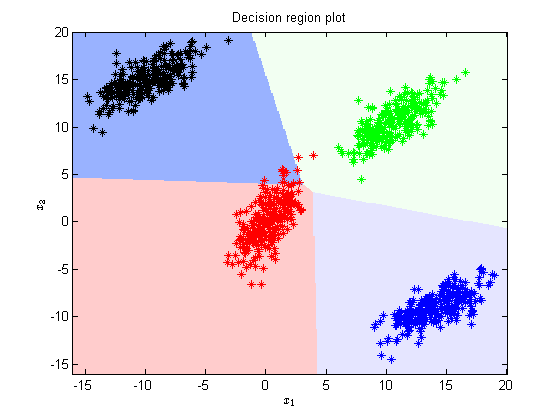
\includegraphics[scale=1]{Classification/1a/c_linear/dec}
\end{center}


The separating hyperplanes obtained were as follows (Support vectors as marked).
\begin{figure}
\begin{subfigure}{.5\textwidth}
  \centering
  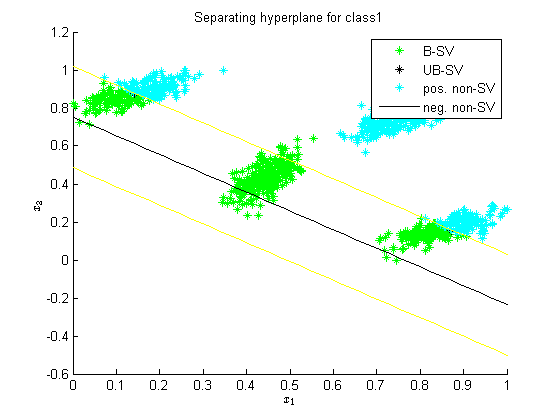
\includegraphics[width=.8\linewidth]{Classification/1a/c_linear/hc1}
 
\end{subfigure}%
\begin{subfigure}{.5\textwidth}
  \centering
  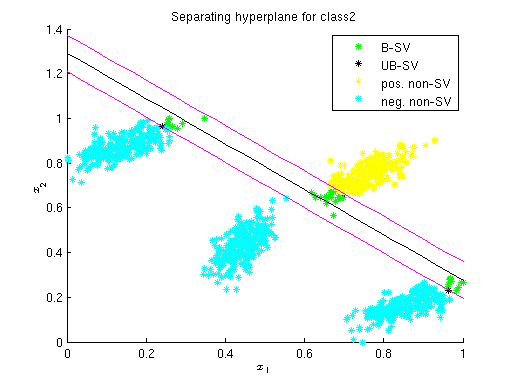
\includegraphics[width=.8\linewidth]{Classification/1a/c_linear/hc2}
  
\end{subfigure}
\end{figure}

\begin{figure}
\begin{subfigure}{.5\textwidth}
  \centering
  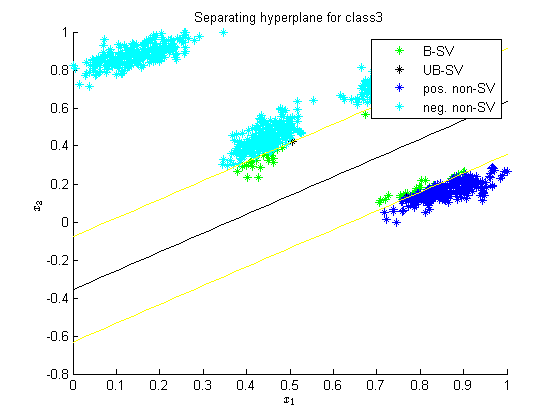
\includegraphics[width=.8\linewidth]{Classification/1a/c_linear/hc3}
 
\end{subfigure}%
\begin{subfigure}{.5\textwidth}
  \centering
  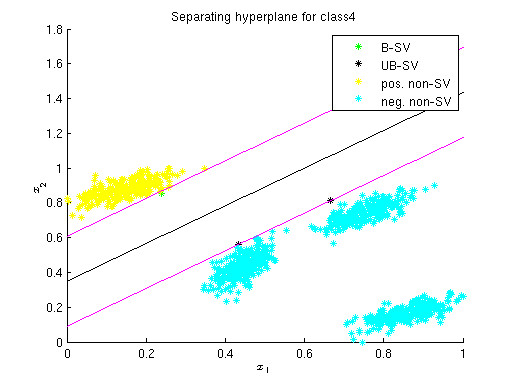
\includegraphics[width=.8\linewidth]{Classification/1a/c_linear/hc4}
  
\end{subfigure}
\end{figure}
\begin{flushleft}
\textbf{Confusion Matrix Train Data\\[5pt]}
\begin{tabular}{|c|c|c|c|}
\hline
237 & 2 & 0 & 11 \\
\hline
0 & 250 & 0 & 0 \\
\hline
0 & 0 & 250 & 0 \\
\hline
0 & 0 & 0 & 250 \\
\hline
\end{tabular}
\textbf{\\[10pt] Confusion Matrix Test Data \\[5pt]}
\begin{tabular}{|c|c|c|c|}
\hline
94 & 1 & 0 & 5 \\
\hline
0 & 100 & 0 & 0 \\
\hline
0 & 0 & 100 & 0 \\
\hline
0 & 0 & 0 & 100 \\
\hline
\end{tabular}
\textbf{\\[10pt] Confusion Matrix Validation Data \\[5pt]}
\begin{tabular}{|c|c|c|c|}
\hline
144 & 0 & 0 & 6 \\
\hline
0 & 150 & 0 & 0 \\
\hline
0 & 0 & 150 & 0 \\
\hline
0 & 0 & 0 & 150 \\
\hline
\end{tabular}
\end{flushleft}




\subsubsection{C-svm with Polynomial Kernel}

Decision Region obtained was as follows.
\begin{center}
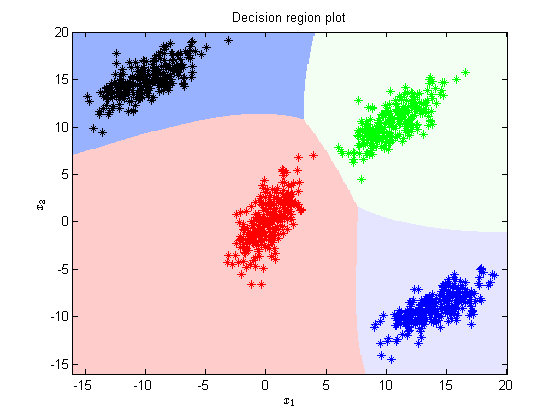
\includegraphics[scale=1]{Classification/1a/c_poly/dec}
\end{center}


The support vectors obtained were as follows.
\begin{figure}
\begin{subfigure}{.5\textwidth}
  \centering
  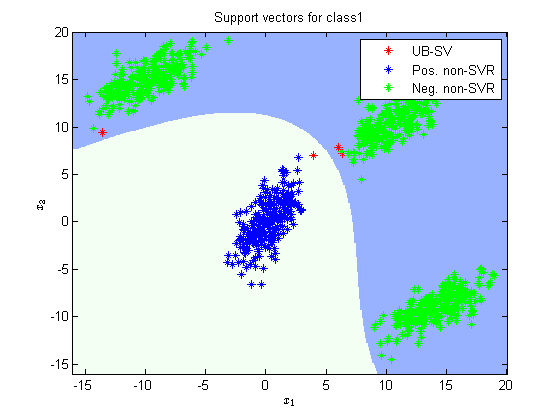
\includegraphics[width=.8\linewidth]{Classification/1a/c_poly/sv1}
 
\end{subfigure}%
\begin{subfigure}{.5\textwidth}
  \centering
  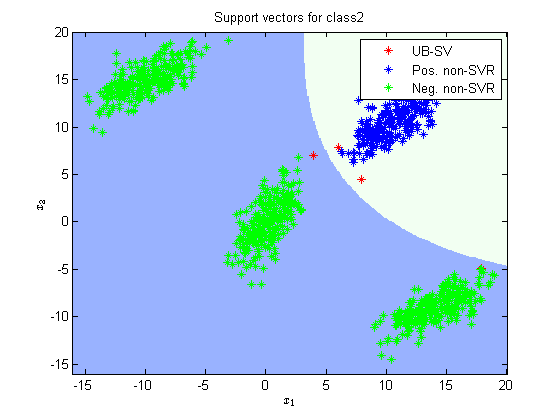
\includegraphics[width=.8\linewidth]{Classification/1a/c_poly/sv2}
  
\end{subfigure}
\end{figure}

\begin{figure}
\begin{subfigure}{.5\textwidth}
  \centering
  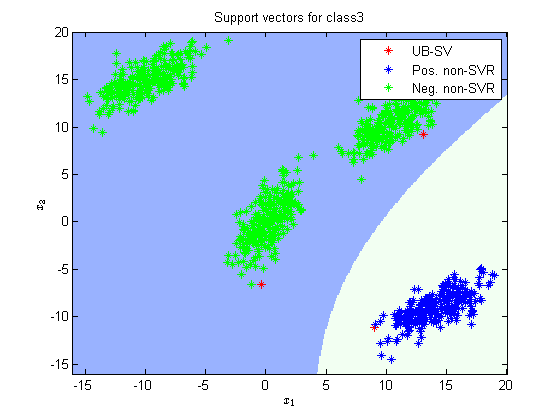
\includegraphics[width=.8\linewidth]{Classification/1a/c_poly/sv3}
 
\end{subfigure}%
\begin{subfigure}{.5\textwidth}
  \centering
  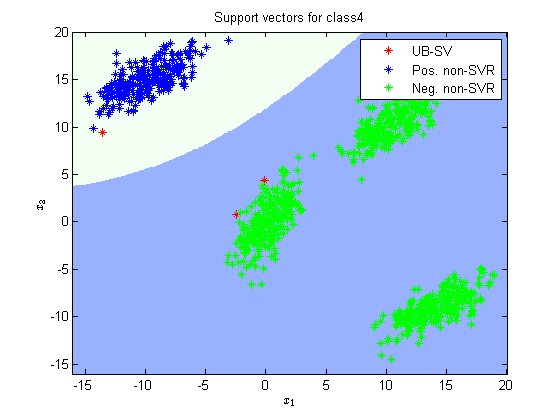
\includegraphics[width=.8\linewidth]{Classification/1a/c_poly/sv4}
  
\end{subfigure}
\end{figure}
\begin{flushleft}
\textbf{Confusion Matrix Train Data\\[5pt]}
\begin{tabular}{|c|c|c|c|}
\hline
250 & 0 & 0 & 0 \\
\hline
0 & 250 & 0 & 0 \\
\hline
0 & 0 & 250 & 0 \\
\hline
0 & 0 & 0 & 250 \\
\hline
\end{tabular}
\textbf{\\[10pt] Confusion Matrix Test Data \\[5pt]}
\begin{tabular}{|c|c|c|c|}
\hline
100 & 0 & 0 & 0 \\
\hline
1 & 99 & 0 & 0 \\
\hline
0 & 0 & 100 & 0 \\
\hline
0 & 0 & 0 & 100 \\
\hline
\end{tabular}
\textbf{\\[10pt] Confusion Matrix Validation Data \\[5pt]}
\begin{tabular}{|c|c|c|c|}
\hline
150 & 0 & 0 & 0 \\
\hline
0 & 150 & 0 & 0 \\
\hline
0 & 0 & 150 & 0 \\
\hline
0 & 0 & 0 & 150 \\
\hline
\end{tabular}
\end{flushleft}


\subsubsection{C-svm with Gaussian Kernel}
Decision Region obtained was as follows.
\begin{center}
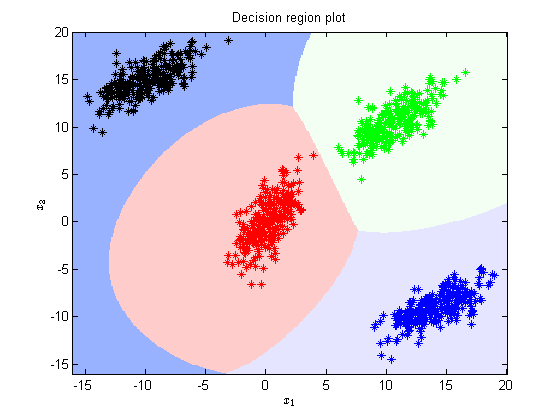
\includegraphics[scale=1]{Classification/1a/c_g/dec}
\end{center}
Support Vector Plots classwise.
\begin{figure}
\begin{subfigure}{.5\textwidth}
  \centering
  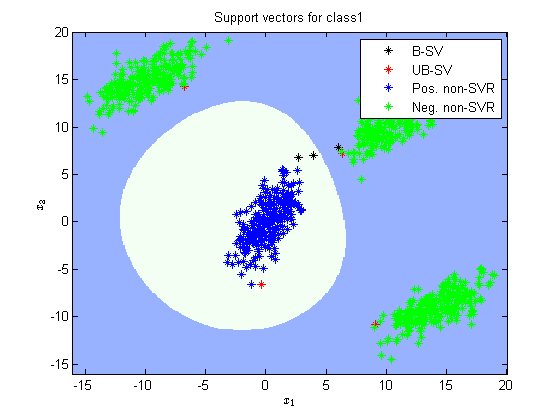
\includegraphics[width=.8\linewidth]{Classification/1a/c_g/svc1}
 
\end{subfigure}%
\begin{subfigure}{.5\textwidth}
  \centering
  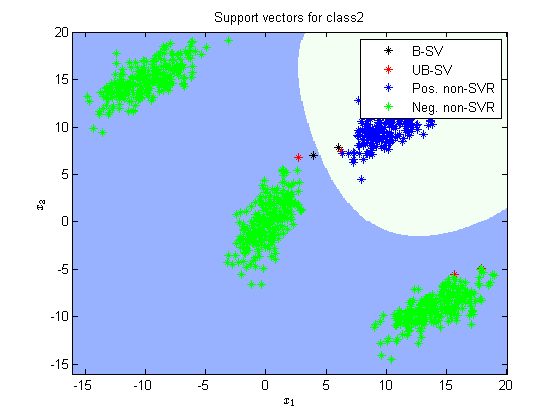
\includegraphics[width=.8\linewidth]{Classification/1a/c_g/svc2}
  
\end{subfigure}
\end{figure}




\begin{figure}
\begin{subfigure}{.5\textwidth}
  \centering
  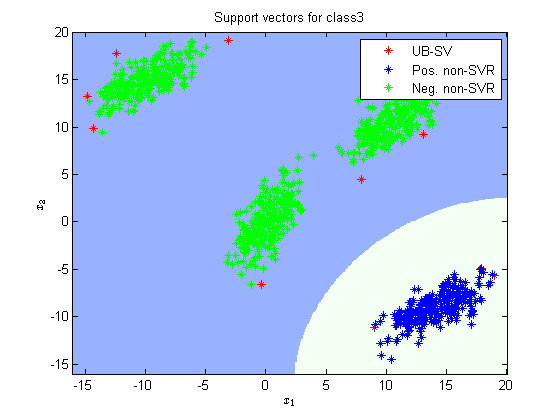
\includegraphics[width=.8\linewidth]{Classification/1a/c_g/svc3}
 
\end{subfigure}%
\begin{subfigure}{.5\textwidth}
  \centering
  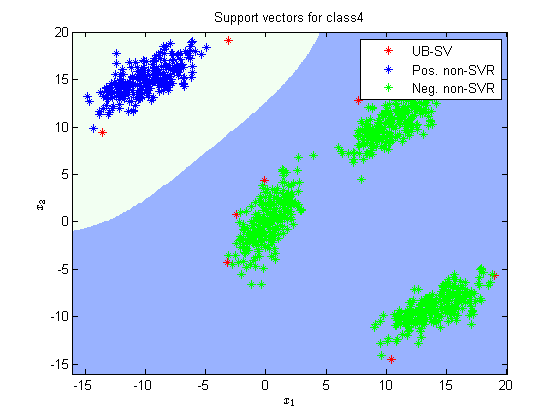
\includegraphics[width=.8\linewidth]{Classification/1a/c_g/svc4}
  
\end{subfigure}
\end{figure}
Kernel Gram matrix for Gaussian Kernel is as follows.
\begin{center}
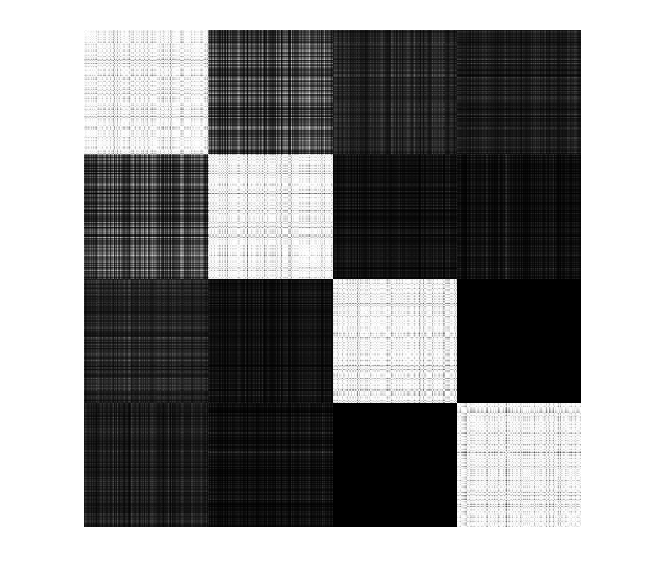
\includegraphics[scale=1]{Classification/1a/c_g/kgm}
\end{center}
\begin{flushleft}
\textbf{Confusion Matrix Train Data\\[5pt]}
\begin{tabular}{|c|c|c|c|}
\hline
250 & 0 & 0 & 0 \\
\hline
0 & 250 & 0 & 0 \\
\hline
0 & 0 & 250 & 0 \\
\hline
0 & 0 & 0 & 250 \\
\hline
\end{tabular}
\textbf{\\[10pt] Confusion Matrix Test Data \\[5pt]}
\begin{tabular}{|c|c|c|c|}
\hline
100 & 0 & 0 & 0 \\
\hline
0 & 100 & 0 & 0 \\
\hline
0 & 0 & 100 & 0 \\
\hline
0 & 0 & 0 & 100 \\
\hline
\end{tabular}
\textbf{\\[10pt] Confusion Matrix Validation Data \\[5pt]}
\begin{tabular}{|c|c|c|c|}
\hline
150 & 0 & 0 & 0 \\
\hline
0 & 150 & 0 & 0 \\
\hline
0 & 0 & 150 & 0 \\
\hline
0 & 0 & 0 & 150 \\
\hline
\end{tabular}
\end{flushleft}


\subsubsection{$\nu$-svm with Gaussian Kernel}
Decision Region obtained was as follows.
\begin{center}
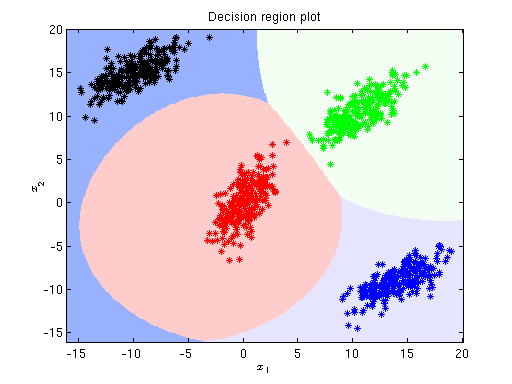
\includegraphics[scale=1]{Classification/1a/nu_g/dec}
\end{center}
Support Vector Plots classwise.
\begin{figure}
\begin{subfigure}{.5\textwidth}
  \centering
  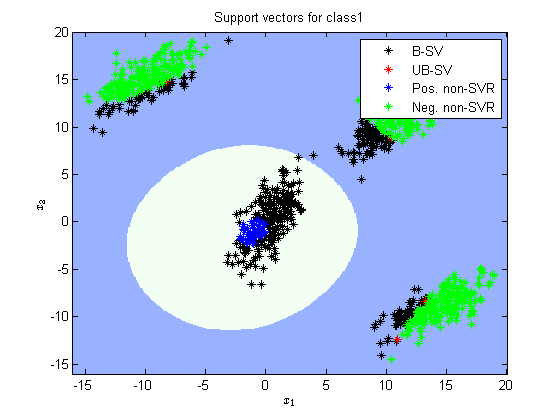
\includegraphics[width=.8\linewidth]{Classification/1a/nu_g/sv1}
 
\end{subfigure}%
\begin{subfigure}{.5\textwidth}
  \centering
  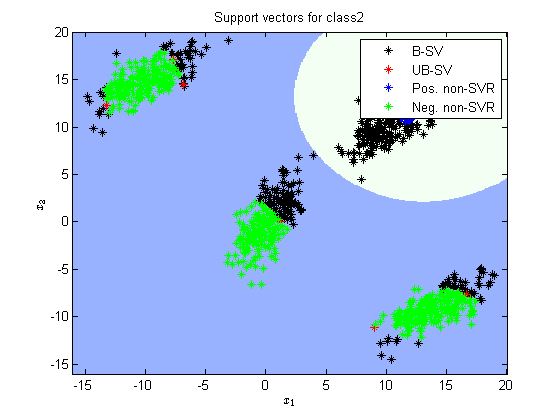
\includegraphics[width=.8\linewidth]{Classification/1a/nu_g/sv2}
  
\end{subfigure}
\end{figure}




\begin{figure}
\begin{subfigure}{.5\textwidth}
  \centering
  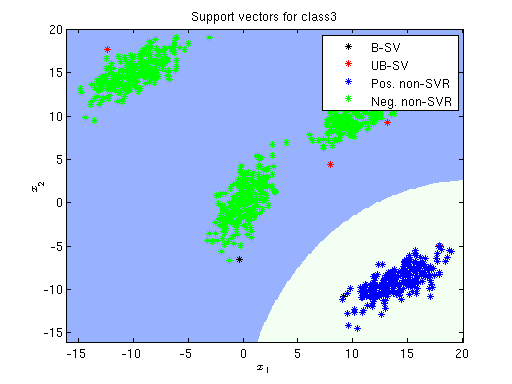
\includegraphics[width=.8\linewidth]{Classification/1a/nu_g/sv3}
 
\end{subfigure}%
\begin{subfigure}{.5\textwidth}
  \centering
  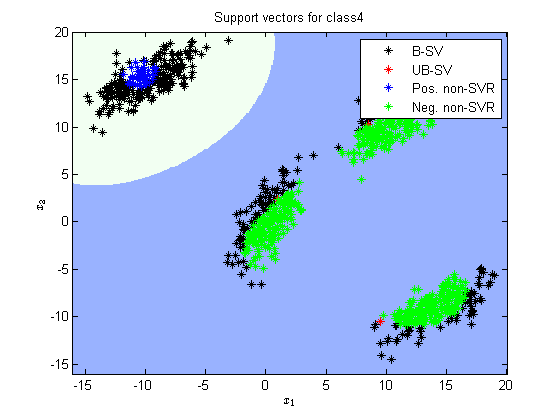
\includegraphics[width=.8\linewidth]{Classification/1a/nu_g/sv4}
  
\end{subfigure}
\end{figure}
Kernel Gram matrix for Gaussian Kernel is as follows.
\begin{center}
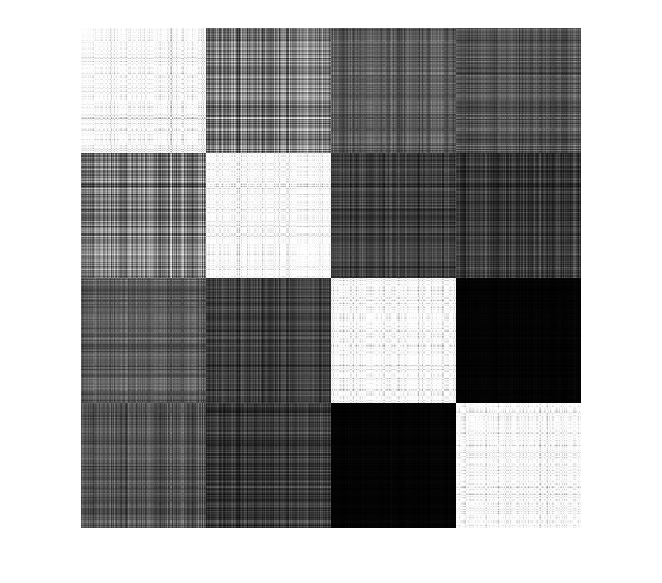
\includegraphics[scale=1]{Classification/1a/nu_g/kgm}
\end{center}
\begin{flushleft}
\textbf{Confusion Matrix Train Data\\[5pt]}
\begin{tabular}{|c|c|c|c|}
\hline
249 & 1 & 0 & 0 \\
\hline
0 & 250 & 0 & 0 \\
\hline
0 & 0 & 250 & 0 \\
\hline
0 & 0 & 0 & 250 \\
\hline
\end{tabular}
\textbf{\\[10pt] Confusion Matrix Test Data \\[5pt]}
\begin{tabular}{|c|c|c|c|}
\hline
100 & 0 & 0 & 0 \\
\hline
0 & 100 & 0 & 0 \\
\hline
0 & 0 & 100 & 0 \\
\hline
0 & 0 & 0 & 100 \\
\hline
\end{tabular}
\textbf{\\[10pt] Confusion Matrix Validation Data \\[5pt]}
\begin{tabular}{|c|c|c|c|}
\hline
150 & 0 & 0 & 0 \\
\hline
0 & 150 & 0 & 0 \\
\hline
0 & 0 & 150 & 0 \\
\hline
0 & 0 & 0 & 150 \\
\hline
\end{tabular}
\end{flushleft}






\subsection{Dataset 1b - Nonlinearly Separable Data}


\subsubsection{C-svm with Polynomial Kernel}

Decision Region obtained was as follows.
\begin{center}
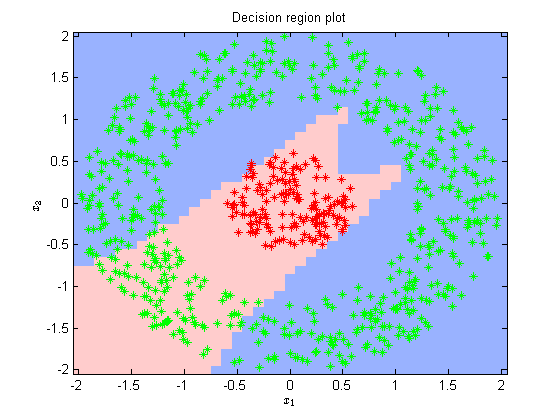
\includegraphics[scale=1]{Classification/1b/c_poly/dec}
\end{center}


The support vectors obtained were as follows.
\begin{figure}
\begin{subfigure}{.5\textwidth}
  \centering
  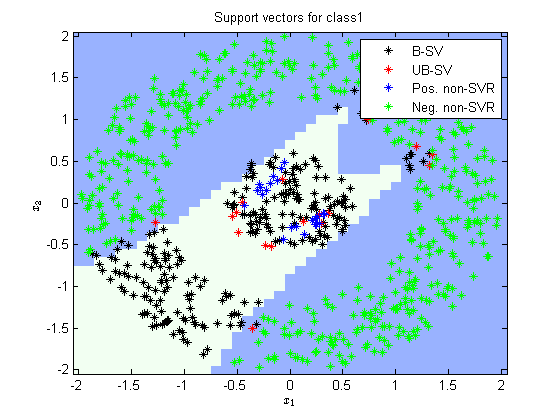
\includegraphics[width=.8\linewidth]{Classification/1b/c_poly/sv1}
 
\end{subfigure}%
\begin{subfigure}{.5\textwidth}
  \centering
  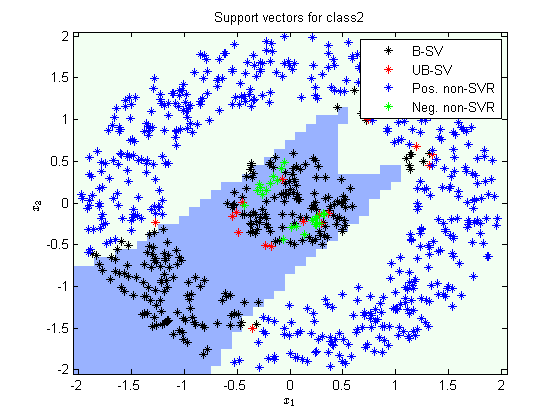
\includegraphics[width=.8\linewidth]{Classification/1b/c_poly/sv2}
  
\end{subfigure}
\end{figure}

\begin{flushleft}
\textbf{Confusion Matrix Train Data\\[5pt]}
\begin{tabular}{|c|c|}
\hline
147 & 3 \\
\hline
99 & 501\\
\hline
\end{tabular}
\textbf{\\[10pt] Confusion Matrix Test Data \\[5pt]}
\begin{tabular}{|c|c|}
\hline
59 & 1 \\
\hline
48 & 192\\
\hline
\end{tabular}
\textbf{\\[10pt] Confusion Matrix Validation Data \\[5pt]}
\begin{tabular}{|c|c|}
\hline
88 & 2 \\
\hline
50 & 310\\
\hline
\end{tabular}
\end{flushleft}


\subsubsection{C-svm with Gaussian Kernel}
Decision Region obtained was as follows.
\begin{center}
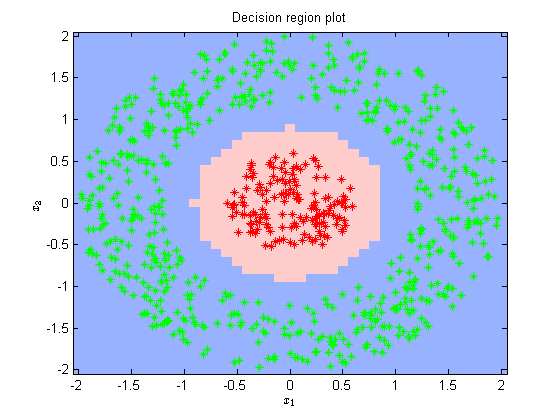
\includegraphics[scale=1]{Classification/1b/c_g/dec}
\end{center}
Support Vector Plots classwise.
\begin{figure}
\begin{subfigure}{.5\textwidth}
  \centering
  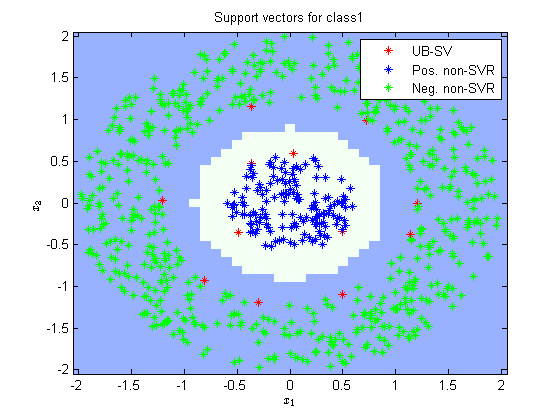
\includegraphics[width=.8\linewidth]{Classification/1b/c_g/sv1}
 
\end{subfigure}%
\begin{subfigure}{.5\textwidth}
  \centering
  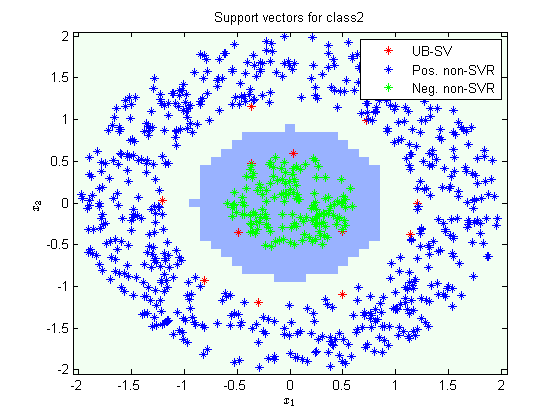
\includegraphics[width=.8\linewidth]{Classification/1b/c_g/sv2}
  
\end{subfigure}
\end{figure}


Kernel Gram matrix for Gaussian Kernel is as follows.
\begin{center}
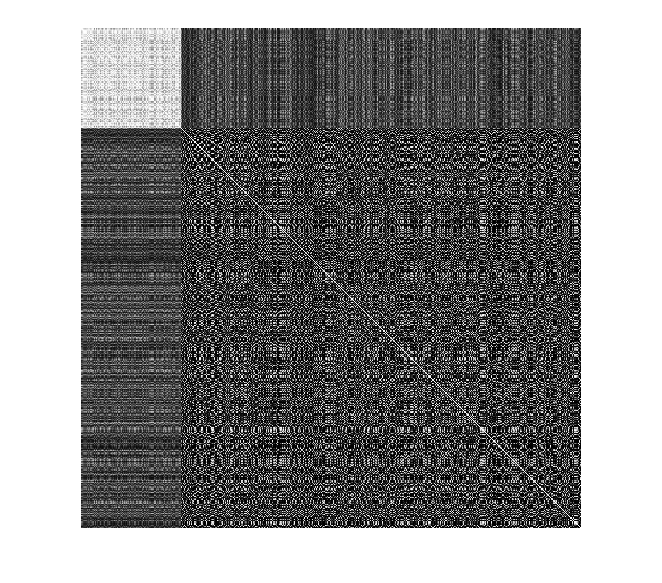
\includegraphics[scale=1]{Classification/1b/c_g/kgm}
\end{center}

\begin{flushleft}
\textbf{Confusion Matrix Train Data\\[5pt]}
\begin{tabular}{|c|c|}
\hline
150 & 0 \\
\hline
0 & 600\\
\hline
\end{tabular}
\textbf{\\[10pt] Confusion Matrix Test Data \\[5pt]}
\begin{tabular}{|c|c|}
\hline
60 & 0 \\
\hline
0 & 240\\
\hline
\end{tabular}
\textbf{\\[10pt] Confusion Matrix Validation Data \\[5pt]}
\begin{tabular}{|c|c|}
\hline
90 & 0 \\
\hline
0 & 360\\
\hline
\end{tabular}
\end{flushleft}






\subsubsection{$\nu$-svm with Gaussian Kernel}
Decision Region obtained was as follows.
\begin{center}
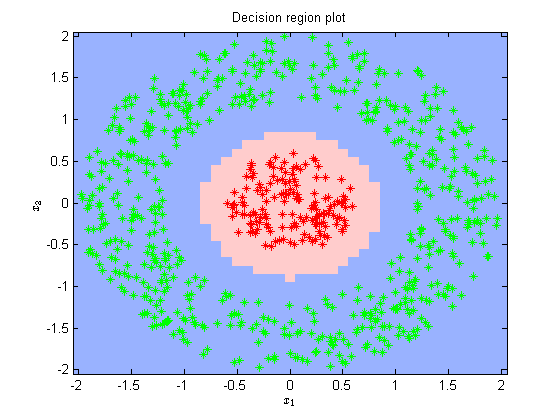
\includegraphics[scale=1]{Classification/1b/nu_g/dec}
\end{center}
Support Vector Plots classwise.
\begin{figure}
\begin{subfigure}{.5\textwidth}
  \centering
  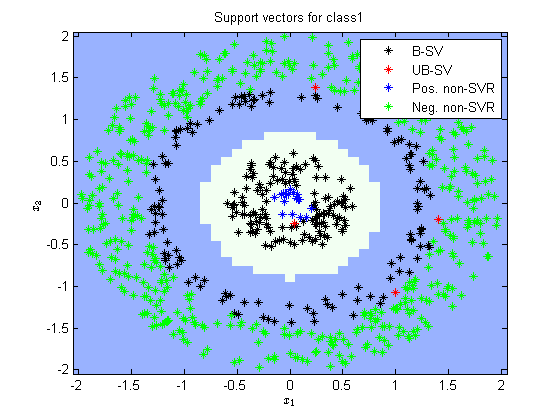
\includegraphics[width=.8\linewidth]{Classification/1b/nu_g/sv1}
 
\end{subfigure}%
\begin{subfigure}{.5\textwidth}
  \centering
  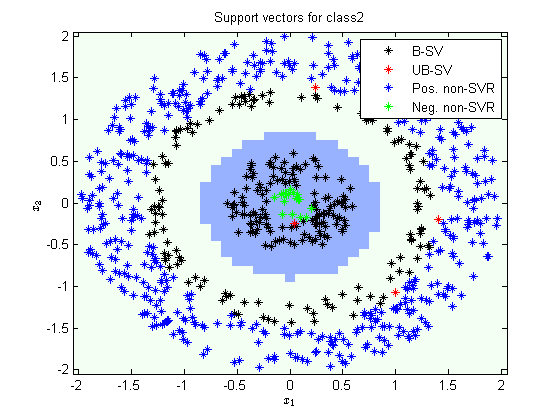
\includegraphics[width=.8\linewidth]{Classification/1b/nu_g/sv2}
  
\end{subfigure}
\end{figure}

Kernel Gram matrix for Gaussian Kernel is as follows.
\begin{center}
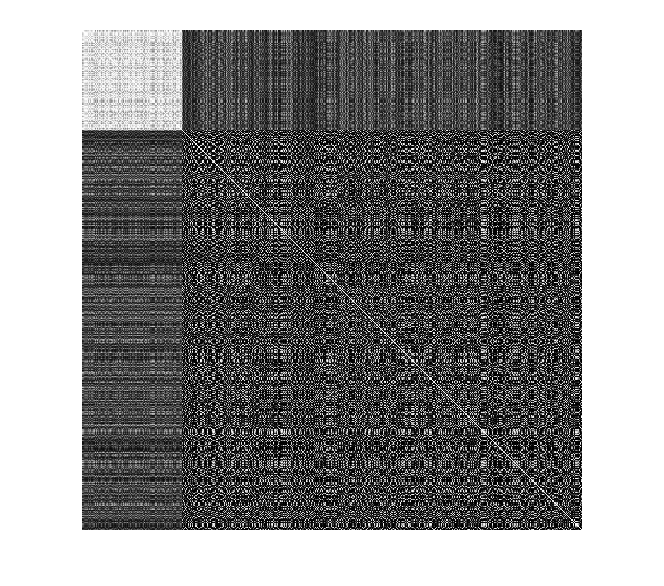
\includegraphics[scale=1]{Classification/1b/nu_g/kgm}
\end{center}


\begin{flushleft}
\textbf{Confusion Matrix Train Data\\[5pt]}
\begin{tabular}{|c|c|}
\hline
150 & 0 \\
\hline
0 & 600\\
\hline
\end{tabular}
\textbf{\\[10pt] Confusion Matrix Test Data \\[5pt]}
\begin{tabular}{|c|c|}
\hline
60 & 0 \\
\hline
0 & 240\\
\hline
\end{tabular}
\textbf{\\[10pt] Confusion Matrix Validation Data \\[5pt]}
\begin{tabular}{|c|c|}
\hline
90 & 0 \\
\hline
0 & 360\\
\hline
\end{tabular}
\end{flushleft}








\subsection{Dataset 1c - Overlapping Data}



\subsubsection{C-svm with Linear Kernel}

Decision Region obtained was as follows.
\begin{center}
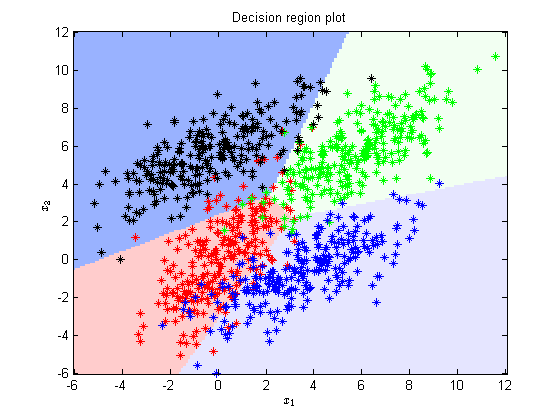
\includegraphics[scale=1]{Classification/1c/c_linear/dec}
\end{center}


The separating hyperplanes obtained were as follows (Support vectors as marked).
\begin{figure}
\begin{subfigure}{.5\textwidth}
  \centering
  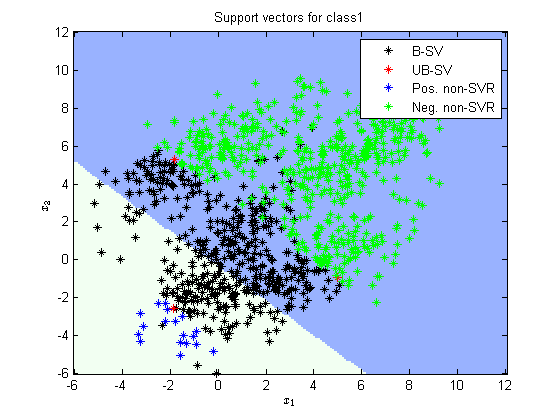
\includegraphics[width=.8\linewidth]{Classification/1c/c_linear/sv1}
 
\end{subfigure}%
\begin{subfigure}{.5\textwidth}
  \centering
  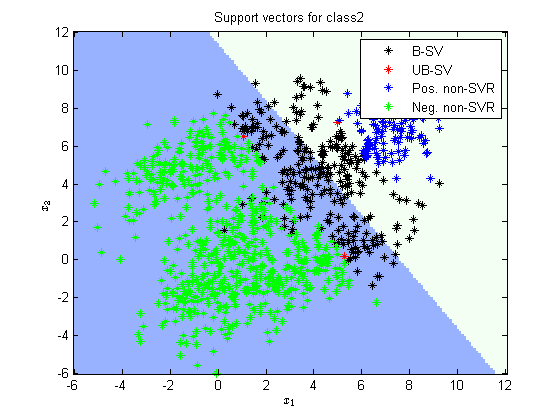
\includegraphics[width=.8\linewidth]{Classification/1c/c_linear/sv2}
  
\end{subfigure}
\end{figure}

\begin{figure}
\begin{subfigure}{.5\textwidth}
  \centering
  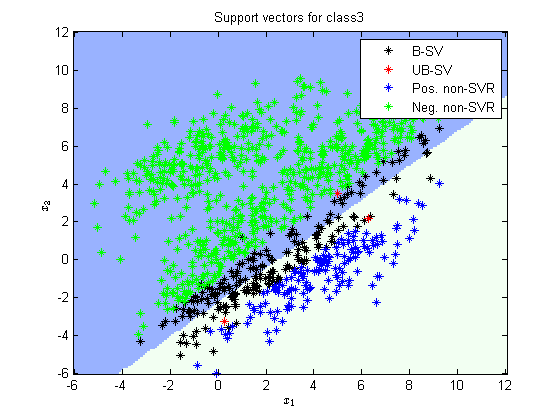
\includegraphics[width=.8\linewidth]{Classification/1c/c_linear/sv3}
 
\end{subfigure}%
\begin{subfigure}{.5\textwidth}
  \centering
  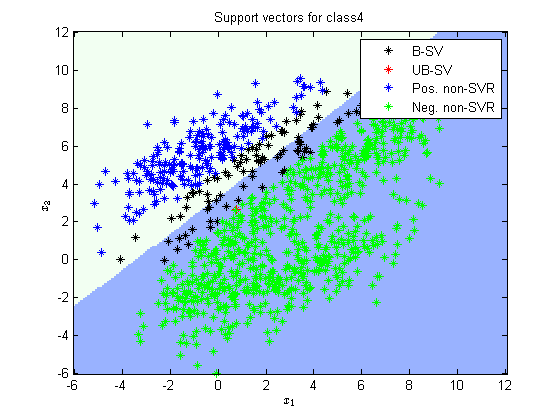
\includegraphics[width=.8\linewidth]{Classification/1c/c_linear/sv4}
  
\end{subfigure}
\end{figure}
\begin{flushleft}
\textbf{Confusion Matrix Train Data\\[5pt]}
\begin{tabular}{|c|c|c|c|}
\hline
209 & 7 & 7 & 17 \\
\hline
6 & 234 & 6 & 4 \\
\hline
27 & 3 & 220 & 0 \\
\hline
1 & 10 & 0 & 239 \\
\hline
\end{tabular}
\textbf{\\[10pt] Confusion Matrix Test Data \\[5pt]}
\begin{tabular}{|c|c|c|c|}
\hline
82 & 1 & 5 & 12 \\
\hline
5 & 88 & 4 & 3 \\
\hline
13 & 2 & 85 & 0 \\
\hline
0 & 0 & 0 & 100 \\
\hline
\end{tabular}
\textbf{\\[10pt] Confusion Matrix Validation Data \\[5pt]}
\begin{tabular}{|c|c|c|c|}
\hline
115 & 3 & 7 & 25 \\
\hline
5 & 133 & 8 & 4 \\
\hline
16 & 3 & 131 & 0 \\
\hline
0 & 5 & 0 & 145 \\
\hline
\end{tabular}
\end{flushleft}

\subsubsection{C-svm with Polynomial Kernel}

Decision Region obtained was as follows.
\begin{center}
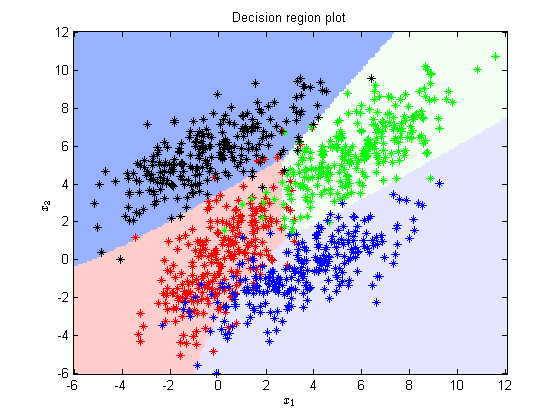
\includegraphics[scale=1]{Classification/1c/c_poly/dec}
\end{center}


The support vectors obtained were as follows.
\begin{figure}
\begin{subfigure}{.5\textwidth}
  \centering
  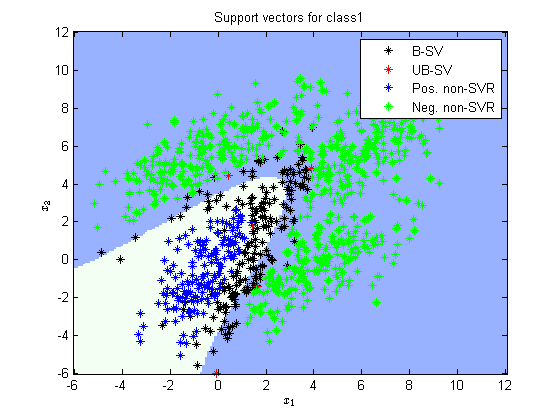
\includegraphics[width=.8\linewidth]{Classification/1c/c_poly/sv1}
 
\end{subfigure}%
\begin{subfigure}{.5\textwidth}
  \centering
  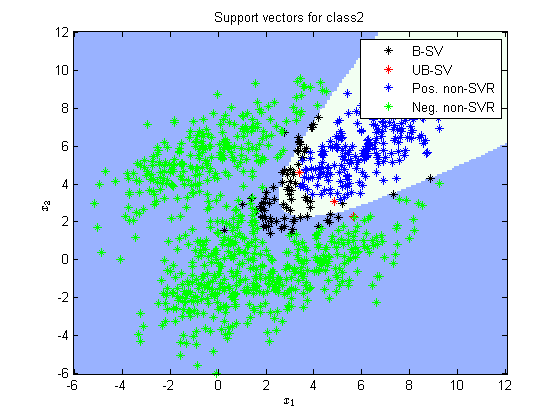
\includegraphics[width=.8\linewidth]{Classification/1c/c_poly/sv2}
  
\end{subfigure}
\end{figure}

\begin{figure}
\begin{subfigure}{.5\textwidth}
  \centering
  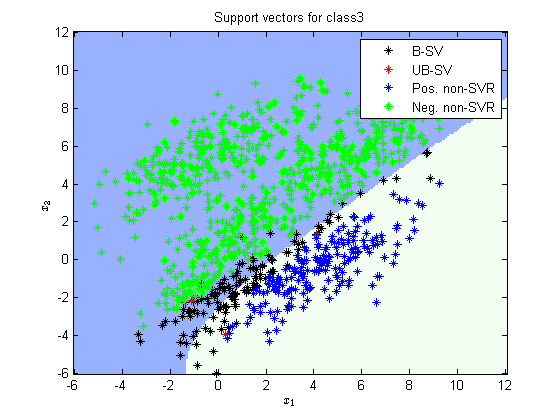
\includegraphics[width=.8\linewidth]{Classification/1c/c_poly/sv3}
 
\end{subfigure}%
\begin{subfigure}{.5\textwidth}
  \centering
  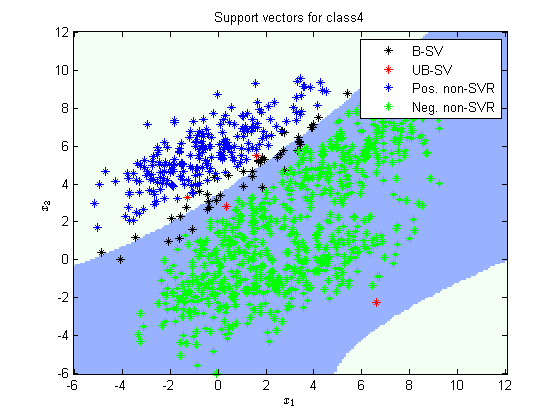
\includegraphics[width=.8\linewidth]{Classification/1c/c_poly/sv4}
  
\end{subfigure}
\end{figure}
\begin{flushleft}
\textbf{Confusion Matrix Train Data\\[5pt]}
\begin{tabular}{|c|c|c|c|}
\hline
221 & 9 & 13 & 7 \\
\hline
8 & 239 & 2 & 1 \\
\hline
28 & 3 & 219 & 0 \\
\hline
4 & 5 & 0 & 241 \\
\hline
\end{tabular}
\textbf{\\[10pt] Confusion Matrix Test Data \\[5pt]}
\begin{tabular}{|c|c|c|c|}
\hline
92 & 2 & 4 & 2 \\
\hline
9 & 86 & 4 & 1 \\
\hline
17 & 4 & 79 & 0 \\
\hline
2 & 0 & 0 & 98 \\
\hline
\end{tabular}
\textbf{\\[10pt] Confusion Matrix Validation Data \\[5pt]}
\begin{tabular}{|c|c|c|c|}
\hline
136 & 1 & 5 & 8 \\
\hline
8 & 137 & 3 & 2 \\
\hline
16 & 1 & 133 & 0 \\
\hline
8 & 2 & 0 & 140 \\
\hline
\end{tabular}
\end{flushleft}



\subsubsection{C-svm with Gaussian Kernel}
Decision Region obtained was as follows.
\begin{center}
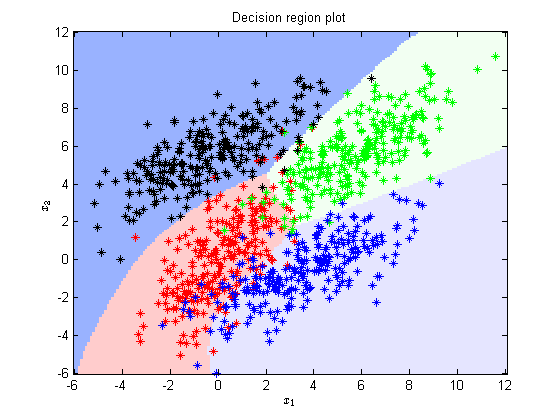
\includegraphics[scale=1]{Classification/1c/c_g/dec}
\end{center}
Support Vector Plots classwise.
\begin{figure}
\begin{subfigure}{.5\textwidth}
  \centering
  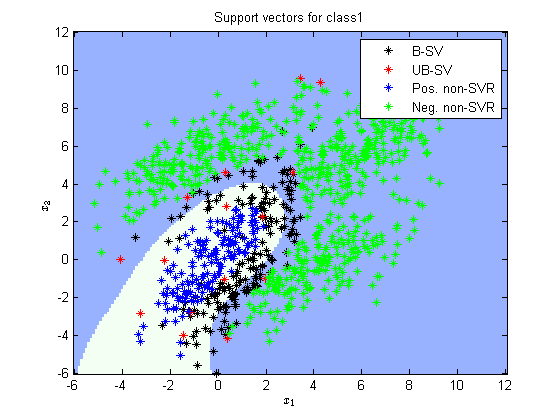
\includegraphics[width=.8\linewidth]{Classification/1c/c_g/sv1}
 
\end{subfigure}%
\begin{subfigure}{.5\textwidth}
  \centering
  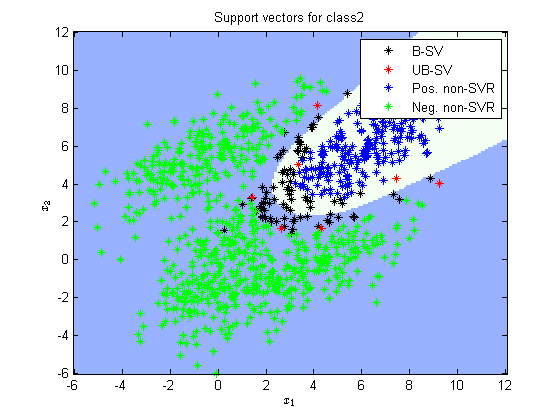
\includegraphics[width=.8\linewidth]{Classification/1c/c_g/sv2}
  
\end{subfigure}
\end{figure}




\begin{figure}
\begin{subfigure}{.5\textwidth}
  \centering
  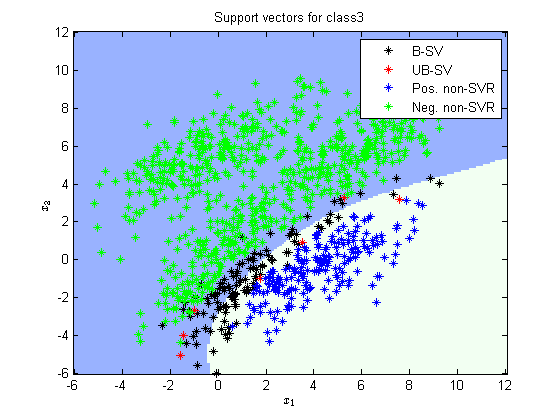
\includegraphics[width=.8\linewidth]{Classification/1c/c_g/sv3}
 
\end{subfigure}%
\begin{subfigure}{.5\textwidth}
  \centering
  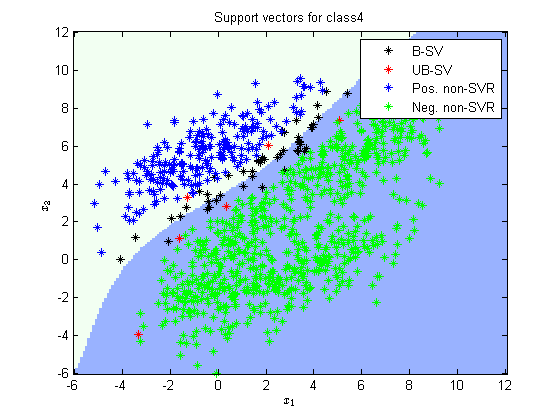
\includegraphics[width=.8\linewidth]{Classification/1c/c_g/sv4}
  
\end{subfigure}
\end{figure}
Kernel Gram matrix for Gaussian Kernel is as follows.
\begin{center}
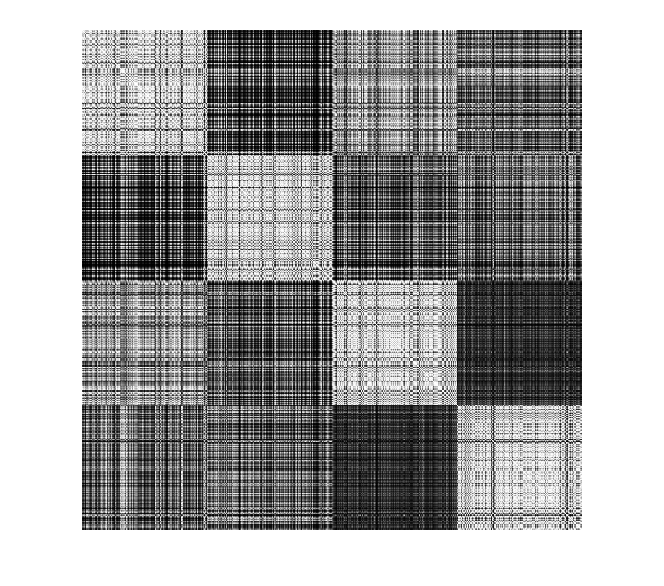
\includegraphics[scale=1]{Classification/1c/c_g/kgm}
\end{center}
\begin{flushleft}
\textbf{Confusion Matrix Train Data\\[5pt]}
\begin{tabular}{|c|c|c|c|}
\hline
216 & 9 & 18 & 7 \\
\hline
9 & 236 & 4 & 1 \\
\hline
24 & 1 & 225 & 0 \\
\hline
1 & 5 & 0 & 244 \\
\hline
\end{tabular}
\textbf{\\[10pt] Confusion Matrix Test Data \\[5pt]}
\begin{tabular}{|c|c|c|c|}
\hline
94 & 1 & 0 & 5 \\
\hline
0 & 100 & 0 & 0 \\
\hline
0 & 0 & 100 & 0 \\
\hline
0 & 0 & 0 & 100 \\
\hline
\end{tabular}
\textbf{\\[10pt] Confusion Matrix Validation Data \\[5pt]}
\begin{tabular}{|c|c|c|c|}
\hline
132 & 4 & 7 & 7 \\
\hline
7 & 139 & 2 & 2 \\
\hline
13 & 1 & 136 & 0 \\
\hline
4 & 5 & 0 & 141 \\
\hline
\end{tabular}
\end{flushleft}



\subsubsection{$\nu$-svm with Gaussian Kernel}
Decision Region obtained was as follows.
\begin{center}
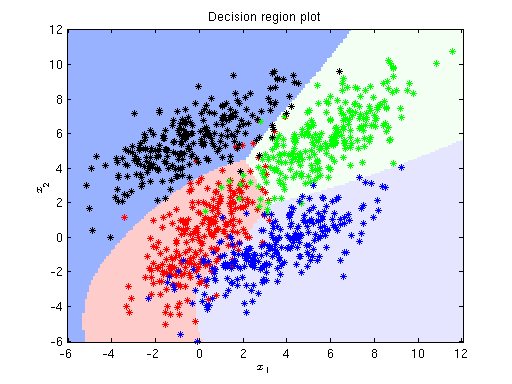
\includegraphics[scale=1]{Classification/1c/nu_g/dec}
\end{center}
Support Vector Plots classwise.
\begin{figure}
\begin{subfigure}{.5\textwidth}
  \centering
  \includegraphics[width=.8\linewidth]{Classification/1c/nu_g/sv1}
 
\end{subfigure}%
\begin{subfigure}{.5\textwidth}
  \centering
  \includegraphics[width=.8\linewidth]{Classification/1c/nu_g/sv2}
  
\end{subfigure}
\end{figure}




\begin{figure}
\begin{subfigure}{.5\textwidth}
  \centering
  \includegraphics[width=.8\linewidth]{Classification/1c/nu_g/sv3}
 
\end{subfigure}%
\begin{subfigure}{.5\textwidth}
  \centering
  \includegraphics[width=.8\linewidth]{Classification/1c/nu_g/sv4}
  
\end{subfigure}
\end{figure}
Kernel Gram matrix for Gaussian Kernel is as follows.
\begin{center}
\includegraphics[scale=1]{Classification/1c/nu_g/kgm}
\end{center}
\begin{flushleft}
\textbf{Confusion Matrix Train Data\\[5pt]}
\begin{tabular}{|c|c|c|c|}
\hline
200 & 16 & 27 & 7 \\
\hline
5 & 243 & 1 & 1 \\
\hline
23 & 2 & 225 & 0 \\
\hline
5 & 8 & 0 & 237 \\
\hline
\end{tabular}
\textbf{\\[10pt] Confusion Matrix Test Data \\[5pt]}
\begin{tabular}{|c|c|c|c|}
\hline
78 & 5 & 11 & 6 \\
\hline
3 & 91 & 4 & 2 \\
\hline
13 & 4 & 83 & 0 \\
\hline
1 & 0 & 0 & 99 \\
\hline
\end{tabular}
\textbf{\\[10pt] Confusion Matrix Validation Data \\[5pt]}
\begin{tabular}{|c|c|c|c|}
\hline
117 & 12 & 13 & 8 \\
\hline
3 & 143 & 3 & 1 \\
\hline
11 & 1 & 138 & 0 \\
\hline
2 & 5 & 0 & 143 \\
\hline
\end{tabular}
\end{flushleft}



\subsection{Dataset 2 - Image Data}
\subsubsection{C-svm with Gaussian Kernel}
Kernel Gram matrix for Gaussian Kernel is as follows.
\begin{center}
\includegraphics[scale=1]{Classification/2/c_g/kgm}
\end{center}
\begin{flushleft}
\textbf{Confusion Matrix Train Data\\[5pt]}
\begin{tabular}{|c|c|c|c|c|}
\hline
113 & 0 & 1 & 0 & 0 \\
\hline
0 & 84 & 1 & 3 & 0 \\
\hline
1 & 4 & 137 & 0 & 0\\
\hline
0 & 0 & 0 & 114 & 0\\
\hline
0 & 0 & 0 & 0 & 261 \\
\hline
\end{tabular}
\textbf{\\[10pt] Confusion Matrix Test Data \\[5pt]}
\begin{tabular}{|c|c|c|c|c|}
\hline
22 & 5 & 4 & 1 & 5\\
\hline
1 & 22 & 6 & 1 & 0 \\
\hline
13 & 6 & 18 & 0 & 11 \\
\hline
0 & 0 & 0 & 37 & 0 \\
\hline
1 & 2 & 1 & 0 & 83 \\
\hline
\end{tabular}
\textbf{\\[10pt] Confusion Matrix Validation Data \\[5pt]}
\begin{tabular}{|c|c|c|c|c|}
\hline
27 & 3 & 7 & 0 & 2 \\
\hline
7 & 18 & 4 & 0 & 0 \\
\hline
12 & 1 & 27 & 3 & 5 \\
\hline
0 & 0 & 0 & 39 & 0 \\
\hline
0 & 2 & 8 & 0 & 77 \\
\hline
\end{tabular}
\end{flushleft}

\subsubsection{$\nu$-svm with Gaussian Kernel}
Kernel Gram matrix for Gaussian Kernel is as follows.
\begin{center}
\includegraphics[scale=1]{Classification/2/nu_g/kgm}
\end{center}
\begin{flushleft}
\textbf{Confusion Matrix Train Data\\[5pt]}
\begin{tabular}{|c|c|c|c|c|}
\hline
111 & 0 & 0 & 3 & 0 \\
\hline
0 & 81 & 1 & 4 & 2 \\
\hline
1 & 6 & 133 & 0 & 2\\
\hline
0 & 0 & 0 & 114 & 0\\
\hline
0 & 0 & 0 & 0 & 261 \\
\hline
\end{tabular}
\textbf{\\[10pt] Confusion Matrix Test Data \\[5pt]}
\begin{tabular}{|c|c|c|c|c|}
\hline
21 & 2 & 5 & 3 & 6\\
\hline
2 & 21 & 4 & 2 & 1 \\
\hline
12 & 6 & 16 & 3 & 11 \\
\hline
0 & 0 & 0 & 37 & 0 \\
\hline
0 & 2 & 1 & 0 & 84 \\
\hline
\end{tabular}
\textbf{\\[10pt] Confusion Matrix Validation Data \\[5pt]}
\begin{tabular}{|c|c|c|c|c|}
\hline
25 & 3 & 7 & 1 & 3 \\
\hline
7 & 17 & 5 & 0 & 0 \\
\hline
11 & 0 & 25 & 5 & 7 \\
\hline
0 & 0 & 0 & 39 & 0 \\
\hline
1 & 0 & 6 & 0 & 80 \\
\hline
\end{tabular}
\end{flushleft}


















\section{Regression Tasks}

\subsection{Dataset 1: 1 dimensional curve fitting data}
\begin{center}
\includegraphics[scale=1]{Regression/univar}
\end{center}
Both $\epsilon$ and $\nu$-SVR with Gaussian Kernels were applied to this dataset.
\subsubsection{$\epsilon$-SVR}
The parameters of interest for $\epsilon$-SVR are $\epsilon$, The value of $\gamma$ in the radial basis function $e^{(-\gamma|u-v|^2)}$ and cost parameter c. They were obtained by performing a grid search on the log scale and changing/narrowing ranges when lowest MSEs were obtained at the borders.
The best values obtained were $\epsilon$ = 0.0625, c = 4 and $\gamma$ = 16. Following are the corresponding plots.
\begin{center}
\includegraphics[scale=1]{Regression/mse}
\end{center}
The MSE shows a low value for small values of $\epsilon$ and then goes up for larger values. Having a large value of $\epsilon$ hurts the MSE since we have a wider tube and do not penalize high errors. However the minimum at $\epsilon$ = 0.0625 can be explained as the value for which the tube is sufficiently large to accommodate noise and obtain a good fit, and at the same time not permitting excessive error.
\begin{center}
\includegraphics[scale=1]{Regression/Plot_1}
\end{center}
Clearly, the approximated function is very close to the true function. The next plot shows the variation with the noisy target outputs.
\begin{center}
\includegraphics[scale=1]{Regression/Plot_2}
\end{center}
The plot below shows the Unbounded support vectors (the blue points) which lie on the $\epsilon$ tube and the Bounded ones outside.
\begin{center}
\includegraphics[scale=1]{Regression/Plot_3}
\end{center}
The following are the scatter plots of target and model output. We can see that the model outputs are very close to the targets. 
\begin{center}
\includegraphics[scale=0.6]{Regression/scatter_train}
\end{center}
\begin{center}
\includegraphics[scale=0.6]{Regression/scatter_test}
\end{center}
\begin{center}
\includegraphics[scale=0.6]{Regression/scatter_val}
\end{center}


\subsubsection{$\nu$-SVR}
In case of a $\nu$-SVR we need to find the parameters $\nu$, c and $\gamma$, latter two being same as in the previous case. Again parameters were found by cross validation in a manner similar to the previous case. \\[5pt]
The best values obtained were $\nu$ = 0.61, c = 16 and $\gamma$ = 16, and using these, $\epsilon$ obtained = 0.0576 which is similar to the previous best value. The purpose of $\nu$ is to tradeoff model complexity vs $\epsilon$ value. Following are the corresponding plots.
\begin{center}
\includegraphics[scale=1]{Regression/nu/mse}
\end{center}
The MSE values here are quite small since the best $\epsilon$ corresponding to each $\nu$ is implicit. A very high value of $\nu$ is restrictive to $\epsilon$, however a very low or 0 $\nu$ allows a choice of relatively large $\epsilon$ without sufficient penalization. Thus both high and very low values of $\nu$ perform poorly.
\begin{center}
\includegraphics[scale=1]{Regression/nu/Plot_1}
\end{center}
Clearly, the approximated function is very close to the true function. The next plot shows the variation with the noisy target outputs.
\begin{center}
\includegraphics[scale=1]{Regression/nu/Plot_2}
\end{center}
The plot below shows the Unbounded support vectors (the blue points) which lie on the $\epsilon$ tube and the Bounded ones outside.
\begin{center}
\includegraphics[scale=1]{Regression/nu/Plot_3}
\end{center}
The following are the scatter plots of target and model output. We can see that the model outputs are very close to the targets. 
\begin{center}
\includegraphics[scale=0.6]{Regression/nu/scatter_train}
\end{center}
\begin{center}
\includegraphics[scale=0.6]{Regression/nu/scatter_test}
\end{center}
\begin{center}
\includegraphics[scale=0.6]{Regression/nu/scatter_val}
\end{center}
Based on the above 2 models, for the univariate data, the performances of the two models are very close and no appreciable difference is seen.

\subsubsection{Performance comparison for Dataset 1}
The following were the final MSEs obtained on Dataset 1 for the test Dataset (Using test data tells us how generalizable the model built is): \\[5pt]
For the $\epsilon$-SVR method with the best parameters, MSE = 0.0092 \\
For the $\nu$-SVR, again with best parameters, MSE = 0.0089 \\[5pt]
Clearly, $\nu$-SVR is performing slightly better than $\epsilon$-SVR. This is because, it trades off model complexity with $\epsilon$ value. This avoids overfitting at the same time tries to balance this with the width of the $\epsilon$ tube.
\subsection{Dataset 2: Bivariate data}
\begin{center}
\includegraphics[scale=1]{Regression/bivar/bivar}
\end{center}
Again, we apply $\epsilon$ and $\nu$ SVRs with Gaussian Kernels to this dataset as well.
\subsubsection{$\epsilon$-SVR}
Again. The parameters needed are $\epsilon$, The value of $\gamma$ in the radial basis function $e^{(-\gamma|u-v|^2)}$ and cost parameter c. Similar to the previous case the best values were found using cross validation. The values obtained were c = 512, $\epsilon$ = 2 and $\gamma$ = 0.0039. The values of $\gamma$ is significantly lower than that of the univariate case, This is due to the increased dimensionality of the data. 
\\[5pt]
The cost parameter c is high indicating that deviations ($\zeta$s) are strictly penalized to produce better results. The value of $\epsilon$ is also higher than the univariate case primarily due to the higher dimensionality.
\begin{center}
\includegraphics[scale=1]{Regression/bivar/eps/mse}
\end{center}
The minima can be seen at $\epsilon$ = 2 which was the chosen value.
\begin{center}
\includegraphics[scale=1]{Regression/bivar/eps/fun}
\end{center}
The above shows the approximated function at the min MSE parameter values.
\\[10pt]
Following are the plots of target and obtained results over the training, test and validation sets.
\begin{center}
\includegraphics[scale=.6]{Regression/bivar/eps/plot_train}
\end{center}
\begin{center}
\includegraphics[scale=.6]{Regression/bivar/eps/plot_test}
\end{center}
\begin{center}
\includegraphics[scale=.6]{Regression/bivar/eps/plot_val}
\end{center}

The scatter plots corresponding to the above results are as follows.
\begin{center}
\includegraphics[scale=.6]{Regression/bivar/eps/scatter_train}
\end{center}
\begin{center}
\includegraphics[scale=.6]{Regression/bivar/eps/scatter_test}
\end{center}
\begin{center}
\includegraphics[scale=.6]{Regression/bivar/eps/scatter_val}
\end{center}
\subsubsection{$\nu$-SVR}
In case of $\nu$-SVR applied to this data, the best parameter values obtained were c = 256, g = 0.0039 and nu = 0.61. The corresponding value of $\epsilon$ was 2.897. Following are the plots corresponding to this.
\begin{center}
\includegraphics[scale=1]{Regression/bivar/nu/mse}
\end{center}
The minima can be seen at $\nu$ = 0.61 which was the chosen value.
\begin{center}
\includegraphics[scale=1]{Regression/bivar/nu/fun}
\end{center}
The above shows the approximated function at the min MSE parameter values.
\\[10pt]
Following are the plots of target and obtained results over the training, test and validation sets.
\begin{center}
\includegraphics[scale=.6]{Regression/bivar/nu/plot_train}
\end{center}
\begin{center}
\includegraphics[scale=.6]{Regression/bivar/nu/plot_test}
\end{center}
\begin{center}
\includegraphics[scale=.6]{Regression/bivar/nu/plot_val}
\end{center}
The scatter plots corresponding to the above results are as follows.
\begin{center}
\includegraphics[scale=.6]{Regression/bivar/nu/scatter_train}
\end{center}
\begin{center}
\includegraphics[scale=.6]{Regression/bivar/nu/scatter_test}
\end{center}
\begin{center}
\includegraphics[scale=.6]{Regression/bivar/nu/scatter_val}
\end{center}

\subsubsection{Comparison of methods for Dataset 2}
The following were the final MSEs obtained on Dataset 2, for the test Dataset: \\[5pt]
For the $\epsilon$-SVR method with the best parameters, MSE = 32.1259 \\
For the $\nu$-SVR, again with best parameters, MSE = 31.9789 \\[5pt]
Again, $\nu$-SVR is performing slightly better than $\epsilon$-SVR. There is however one difference that we notice, in the case of univariate data, the $\nu$-SVR made $\epsilon$ slightly smaller that the $\epsilon$-SVR whereas here we observe the reverse trend. The larger $\epsilon$ margin here in $\nu$-SVR is actually improving generalizability due to the nature of the data distribution.

















\section{Novelty Detection Tasks}

\subsection{Bivariate Dataset}
\begin{center}
\includegraphics[scale=.6]{SVDD/bivar}
\end{center}
The above shows the unnormalized data, we have normalized it using Min-Max normalization for using in SVDD. For Novelty Detection, Class 1 which is the Blue colored class in the above figure has been set as the positive class.



\subsubsection{c-SVDD}

The parameters of interest here are c, the cost associated with the $\zeta$s and $\gamma$, the inverse of the scale factor in the gaussians. We found them in a manner similar to SVRs using grid search on log scale and narrowing the range using cross validation. Following are the corresponding plots. \\[10pt]
Plot of bounded and unbounded support vectors is as follows.
\begin{center}
\includegraphics[scale=1]{SVDD/c/SV}
\end{center}
The following plots show us the correctly and incorrectly classified points for train, test and val datasets.
\begin{center}
\includegraphics[scale=.8]{SVDD/c/train_plot}
\end{center}
\begin{center}
\includegraphics[scale=.8]{SVDD/c/test_plot}
\end{center}
\begin{center}
\includegraphics[scale=.8]{SVDD/c/val_plot}
\end{center}
The statistics are as follows:\\[5pt]
\textbf{Train data\\}
Total number of points = 250(all are points of +1 class of course) \\
Number of false negatives = 17 (+1 but tagged as -1) = 17/250 = 6.8\% \\  
Correctly classified as +1 = 233 = 93.2\%\\[10pt]
\textbf{Test data\\}
Total number of points = 400 \\
Number of false positives (-1 but tagged as +1) = 48/400 = 12\%\\ 
Number of false negatives (+1 but tagged as -1) = 8/400 = 2\% \\  
Correctly classified = 86\%\\[10pt]
\textbf{Val data\\}
Total number of points = 600 \\
Number of false positives (-1 but tagged as +1) = 46/600 = 7.67\%\\ 
Number of false negatives (+1 but tagged as -1) = 15/600 = 2.5\% \\  
Correctly classified = 89.83\%\\[10pt]

We notice that the number of false positives is higher and false negatives are less. This means that the region built is covering almost all points of class 1 but as expected including some other class points also since the dataset has a lot of overlap.






\subsubsection{$\nu$-SVDD}
The parameters of interest here are $\nu$s and $\gamma$, the inverse of the scale factor in the gaussians. We have used a one class $\nu$-SVM to perform $\nu$-SVDD. The reason why we can do this is that the boundary that is obtained when a SMH is built over a normalized Gaussian Kernel, results in a linear decision boundary which is equivalent to that obtained by using one class $\nu$-SVM. \\[10pt]
Plot of bounded and unbounded support vectors is as follows.
\begin{center}
\includegraphics[scale=1]{SVDD/nu/SV}
\end{center}
The following plots show us the correctly and incorrectly classified points for train, test and val datasets.
\begin{center}
\includegraphics[scale=.8]{SVDD/nu/train_plot}
\end{center}
\begin{center}
\includegraphics[scale=.8]{SVDD/nu/test_plot}
\end{center}
\begin{center}
\includegraphics[scale=.8]{SVDD/nu/val_plot}
\end{center}
The statistics are as follows:\\[5pt]
\textbf{Train data\\}
Total number of points = 250(all are points of +1 class of course) \\
Number of false negatives = 41 (+1 but tagged as -1) = 41/250 = 16.4\% \\  
Correctly classified as +1 = 209 = 83.6\%\\[10pt]
\textbf{Test data\\}
Total number of points = 400 \\
Number of false positives (-1 but tagged as +1) = 31/400 = 7.75\%\\ 
Number of false negatives (+1 but tagged as -1) = 21/400 = 5.25\% \\  
Correctly classified = 87\%\\[10pt]
\textbf{Val data\\}
Total number of points = 600 \\
Number of false positives (-1 but tagged as +1) = 29/600 = 7.25\%\\ 
Number of false negatives (+1 but tagged as -1) = 29/600 = 7.25\% \\  
Correctly classified = 89.83\%\\[10pt]


\subsubsection{Comparison of c and $\nu$-SVDD for Bivariate Dataset}
The final accuracy of both the methods is comparable (86\% and 87\% on the test data). However we notice that the percentage of false positives and false negatives is more balanced in the case of $\nu$-SVDD whereas false positives are significantly higher in case of c-SVDD. \\[5pt]$\nu$-SVDD does a better job of preventing overfitting to the training data. This can be seen from the fact that it does not do as well on the training data as c-SVDD but is slightly better everywhere else.

\subsection{Multivariate Dataset}
This dataset is 13 dimensional and has a total of 297 points which were split across train, test and validation datasets. 
\subsubsection{c-SVDD} 
The statistics are as follows:\\[5pt]
\textbf{Train data\\}
Total number of points = 96(all are points of +1 class of course) \\
Number of false negatives = 23 (+1 but tagged as -1) = 23/96 = 23.95\% \\  
Correctly classified as +1 = 209 = 76.05\%\\[10pt]
\textbf{Test data\\}
Total number of points = 161 \\
Number of false positives (-1 but tagged as +1) = 10/161 = 6.2\%\\ 
Number of false negatives (+1 but tagged as -1) = 29/161 = 18\% \\  
Correctly classified = 75.8\%\\[10pt]
\textbf{Val data\\}
Total number of points = 81 \\
Number of false positives (-1 but tagged as +1) = 4/81 = 4.9\%\\ 
Number of false negatives (+1 but tagged as -1) = 19/81 = 23.4\% \\  
Correctly classified = 71.7\%\\[10pt]

\subsubsection{$\nu$-SVDD} 
The statistics are as follows:\\[5pt]
\textbf{Train data\\}
Total number of points = 96(all are points of +1 class of course) \\
Number of false negatives = 24 (+1 but tagged as -1) = 24/96 = 25\% \\  
Correctly classified as +1 = 209 = 75\%\\[10pt]
\textbf{Test data\\}
Total number of points = 161 \\
Number of false positives (-1 but tagged as +1) = 18/161 = 11.2\%\\ 
Number of false negatives (+1 but tagged as -1) = 17/161 = 10.56\% \\  
Correctly classified = 78.24\%\\[10pt]
\textbf{Val data\\}
Total number of points = 81 \\
Number of false positives (-1 but tagged as +1) = 10/81 = 12.3\%\\ 
Number of false negatives (+1 but tagged as -1) = 22/81 = 27.1\% \\  
Correctly classified = 70.6\%\\[10pt]


\subsubsection{Comparison of c and $\nu$-SVDD for Bivariate Dataset}
Again $\nu$-SVDD is more balanced wrt FPs and FNs. But on the whole, There is no clear or appreciable difference here between the two models. $\nu$-SVDD performed better on the test data, but c-SVDD was slightly better on the validation data. 
\end{document}